\subsubsection{\stid{4.15} UnifyFS -- A file system for burst buffers} 

\paragraph{Overview} 

The view of storage systems for HPC is changing rapidly. Traditional, 
single-target parallel file systems have reached their cost-effective 
scaling limit. As a result, hierarchical storage systems are being designed 
and installed for our nation's next-generation leadership class systems. 
Current designs employ “burst buffers” as a fast cache between compute 
nodes and the parallel file system for data needed by running jobs and 
workflows. Burst buffers are implemented as compute-node local storage 
(e.g., SSD) or as shared intermediate storage (e.g., SSD on shared burst 
buffer nodes).

Because burst buffers present an additional complexity to effectively
using supercomputers, we developed UnifyFS, a user-level file system, 
highly-specialized for shared file access on HPC systems with distributed 
burst buffers.  UnifyFS addresses a major usability 
factor of current and future systems, because it enables
applications to gain the performance advantages from distributed burst buffers 
while providing ease of use similar to that of a parallel file system.
To use UnifyFS from within an MPI application, one only needs to change 
the paths for files that the application uses from the parallel file system 
to the mount point for UnifyFS, \texttt{/unifyfs}. Then the application
performs I/O as it normally would, using POSIX I/O or a high level I/O library, e.g.,
HDF5 or MPI-IO. The UnifyFS library intercepts all I/O operations and 
manages the file data locally on the compute nodes with high performance.

\begin{figure}[htb]
        \centering
        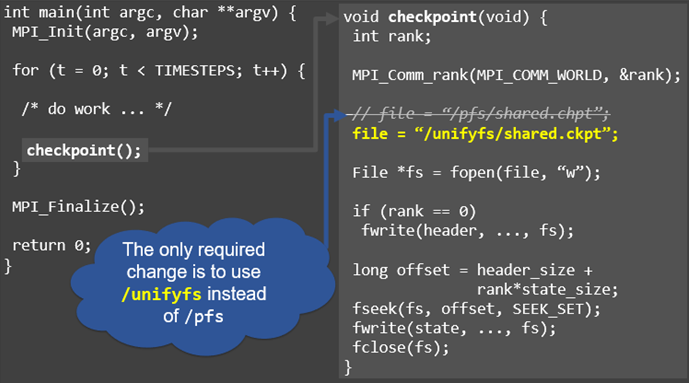
\includegraphics[width=3.5in]{projects/2.3.4-DataViz/2.3.4.15-HDF5-UnifyCR/usingUnifyFS}
        \caption{\label{fig:usingUnifyFS} \textbf{Using UnifyFS} 
Using UnifyFS from an MPI application is as easy as using the parallel file system. 
Simply change the file path to point to the UnifyFS mount point \texttt{/unifyfs}, and
then perform I/O as normal.} 
\end{figure}


\paragraph{Key  Challenges}

The hierarchical storage of current and future HPC systems includes compute-node
local SSDs as burst buffers. This distributed burst buffer design promises
fast, scalable I/O performance because burst buffer bandwidth and capacity
will automatically scale with the compute resources used by jobs and
workflows. However, a major concern for this distributed design is how to
present the disjoint storage devices as a single storage location to
applications that use shared files. The primary issue is that when concurrent
processes on different compute nodes perform I/O operations, e.g., writes,
to a shared file, the data for the file are scattered across the separate
compute-node local burst buffers instead of being stored in a single
location. Consequently, if a process wants to access bytes from the
shared file that exist in the burst buffer of a different compute node,
that process needs to somehow track or look up the information for locating
and retrieving those bytes. Additionally, there is no common interface across
vendors for accessing remote burst buffers, so code for cross-node file
sharing will not be easily portable across multiple DOE systems with
different burst buffer architectures, further increasing programming
complexity to support shared files.

For the reasons outlined above, it is clear that without software support 
for distributed burst buffers, applications
will have major difficulties utilizing these resources. 

\begin{figure}[htb]
        \centering
        %\includegraphics[width=3.5in]{projects/2.3.4-DataViz/2.3.4.15-HDF5-UnifyFS/UnifyFS-overview}
        \includegraphics[width=3.5in]{projects/2.3.4-DataViz/2.3.4.15-HDF5-UnifyCR/UnifyFS-overview}
        \caption{\label{fig:UnifyFS-overview} \textbf{UnifyFS Overview.} Users can give commands in their batch scripts to launch UnifyFS within
their allocation. UnifyFS works transparently with POSIX I/O, common I/O libraries, and
VeloC. Once file operations are intercepted by UnifyFS, they
are handled with specialized optimizations to ensure high performance.}
\end{figure}

\paragraph{Solution Strategy}

To address this concern, we have developed UnifyFS, a user-level file system,
highly-specialized for shared file access on HPC systems with distributed
burst buffers. In Figure \ref{fig:UnifyFS-overview}, we show a high
level schematic of how UnifyFS works. Users load UnifyFS into
their jobs from their batch scripts. Once UnifyFS is instantiated, user
applications can read and write shared files to the mount point just like
they would the parallel file system. File operations to the UnifyFS
mount point will be intercepted and handled with specialized optimizations
that will deliver high I/O performance. 

Because bulk-synchronous I/O dominates the 
I/O traffic most HPC systems, we target our approach at
those workloads. Examples of bulk-synchronous I/O include checkpoint/restart
and periodic output dumps by applications. Thus, UnifyFS  addresses a major usability
factor of current and future systems. We designed UnifyFS such
that it transparently intercepts I/O calls, so it will integrate
cleanly with other software including I/O and checkpoint/restart libraries.
Additionally, because UnifyFS is tailored for HPC systems and workloads,
it can deliver high performance.



\paragraph{Recent Progress}

In the past year, the UnifyFS team has focused on improving the usability
and performance of UnifyFS for applications and I/O middleware.
We evaluated UnifyFS for use by producer-consumer applications, which include
applications such as climate models that exchange data files between independent
components such as ``ocean'' and ``atmosphere'', and applications that couple
traditional HPC simulation with ML analysis. We updated UnifyFS to better support
these types of applications, including documentation additions and fixes to the
UnifyFS code base. This year, we also introduced our UnifyFS API which is intended
to be used by I/O middleware software, e.g., I/O libraries like HDF5. By using this
API, I/O middleware can have finer control over the workings of UnifyFS and obtain
better performance. Finally, we also implemented numerous changes and bug fixes
in preparation for our support of UnifyFS on Frontier. 
Our source code for UnifyFS is available on 
GitHub at \url{https://github.com/LLNL/UnifyFS}. Within the last year, we have also deployed UnifyFS on Summit as a production ready module. 

%\begin{figure}[htb]
        %\centering
        %%\includegraphics[width=4in]{projects/2.3.4-DataViz/2.3.4.15-HDF5-UnifyFS/milestone2}
        %\includegraphics[width=4in]{milestone2}
        %\caption{\label{fig:milestone2} \textbf{UnifyFS Design.} The UnifyFS
%instance consists of a dynamic library and a UnifyFS daemon that runs
%on each compute node in the job. The library intercepts I/O calls to
%the UnifyFS mount point from applications, I/O libraries, or VeloC and communicates them to the UnifyFS daemon that handles the I/O operation.}
%\end{figure}
%

\paragraph{Next Steps}

Our efforts for the next year will be focused on delivering a robust and 
high-performance implementation of UnifyFS on Frontier. We have begun the work
of porting to early access systems for Frontier and will continue on this track. 
We will rigorously test the correctness and performance of UnifyFS and will
evaluate UnifyFS's performance with ECP applications on Frontier.

